\documentclass[10pt,conference,compsocconf,retainorgcmds]{IEEEtran}

\usepackage{hyperref}
\usepackage{graphicx}   % For figure environment
\usepackage{color}
\usepackage{natbib}
\usepackage{float}
\usepackage{cprotect}
\usepackage{tabularx}
\usepackage{multirow}
\usepackage{amsmath}
\usepackage{amssymb}
\usepackage{enumitem}

\begin{document}
\title{Text analysis: Machine Learning Project 2}

\author{
  Robin Clerc, Pierre Vigier, Jacob Levy Abitbol\\
  \textit{MSc  Computer Science, EPFL, Switzerland}
}

\maketitle

\begin{abstract}
As microblogging services like Twitter are becoming
more and more influential in today’s globalized world, its facets
like sentiment analysis are being extensively studied. The sheer volume of data produced daily by its users as well as its overall availability, enable researchers to study this classification problem over massive datasets of messages or tweets. The information collected is however inherently noisy, as phenomena such as linguistic drift are known to be sped up over these social media platforms, therefore hindering the use of standard NLP tools. We present here a combined methodology overcoming some of these issues by training a model to predict whether any given tweet is more likely to contain a happy rather than a sad emoji. Specifically, we show how different pre-processing schemes and text embedding (GloVe, word2vec) methods are crucial in driving up the quality of the  predictions yielded by our models. We eventually achieve accuracies of around 86.54\% on an already pre-processed dataset of around 2.5 million labeled tweets by aggregating several approaches.
\end{abstract}








\section{Introduction}
Sentiment classification is the task of detecting whether a textual item expresses an overall positive or negative opinion in general or about a given entity (products, person, policy).
Recently, the advent of social media and publicly available communication platforms has opened up a new gate to access individual information at a massive scale. Among all available social platforms, Twitter has been regarded as the choice by default, namely thanks to the intrinsic nature of communications taking place through it and the existence of data providers that are able to supply researchers with the volume of data they require. It is therefore not surprising that interest in studying sentiment classification through this social platform has grown in recent years. We here study a variant of the original sentiment classification problem by training a model to be able to detect whether a tweet contains  a  happy or sad emoji ( ':)' and  ':('   respectively).

\section{Data Description}
 \label{sec:structure-paper}
\subsection{Data Exploration and Preprocessing: text normalization}

Our dataset consists of a large data corpus collected from the online news and social networking service, Twitter. On it, users can post and interact with messages, "tweets", restricted to 140 characters. Specifically, we are given a sentiment-labeled dataset of 2.5 million tweets, each containing exclusively a happy or sad emoji.  Class imbalance is not an issue in the provided dataset as each sentiment class contains an even number of samples to train our models on (1.25 million for each). Metadata generally contained in the tweets is here preprocessed and indicated by some user defined tag (\textless  mention\textgreater  for @user, \textless hashtag\textgreater  for \#,...).\\

When considering what kind of preprocessing to perform on our dataset, one must first acknowledge the inherently different style of communication used though this service.  Twitter posts are for instance much shorter than in any other traditional media like blogs, as they are constrained by a hard 140 character limit. This is believed to be the cause behind the high compactness and brevity of language in Twitter. Furthermore, it contains highly non-standard orthography alongside a wide range of linguistic variation leading to several non-standard spellings of the same word and hindering the use of standard NLP tools such as tokenizer or stemmers. Keeping those words makes the dimensionality of the problem high and hence the classification more difficult since each word in the text is treated as one dimension. A logical first step would then be to reduce this intrinsic variability by filtering out infrequent word occurrences.

We proceeded to use the preprocessing scheme developed by the Stanford NLP section over a corpus of 2 billions of tweets. The interest here is two-fold: on the one hand,  having trained their methods on such a large corpus enable us to have a general set of rules to deal with exceptions that we otherwise would have had to look for in our corpus. On the other hand, relying on the same preprocessing backbone will in time, allow us to use higher level features (embeddings) developed by this group and computed over their Twitter dataset. The Ruby preprocessing script was hence translated intro Python and adapted to our already tokenized and lower-case proprocessed dataset. We here list its main features:

\begin{itemize}[label={},leftmargin=*]
    \item \textbf{Contractions expanded:} As previously stated, Twitter hard character limit incentivizes the use of contraction of words that are already common in informal text communications: \textit{"I'll've" $\rightarrow$ "I will have"}. Abbreviations are also dealt with in an analogous manner.
    \item \textbf{Hashtag split:} Hashtags come in the form of one or more concatenated words preceded b the \# character. These tokens can in some cases convey additional information that might be useful to perform sentiment analysis (e.g, \#hatetrump, \#loveobama). Although tokenizing a cleansed hashtag can prove quite hard, we assumed that most hashtags are made of a single token and considered it as a given word:\textit{ \#love$\rightarrow$ love, \#savethedate $\rightarrow$ savethedate}. Preprocessing of our data unfortunately prevents us from actually using this step.
    
    \item \textbf{Spell check}: Typos naturally present in the tweets are partially corrected via the edit distance (insertion, deletion, substitution)  to standard words found in online dictionaries. The application of this filter was restricted by the correction speed and the volume of the data we were dealing with : \textit{piercin $\rightarrow$ piercing}. We also introduced some user-defined rules in order to account for frequently observed typos such as character repetitions , where characters observed more than twice are set to be repeated only twice: \textit{gooooood $\rightarrow$ good, honeeeyyy $\rightarrow$ honeeyy}
   \end{itemize}

It is also worth mentioning that some standard NLP preprocessing techniques were tried but finally excluded from the final pipeline such as stopwords removal, which was found to be decreasing the prediction accuracy, part-of-speech tagging which wasn't found to increase our final prediction score. \\
It should also be said that the order in which the preprocessing stages are concatenated is crucial to the overall performance of our model (for instance, letter repetitions should be removed before checking whether a given word is in the dictionary or not). The cleansed dataset is then shuffled in order to mix positive and negative samples during training and testing. We now need to find a way to feed to our learning algorithm a numerical representation of the text it's supposed to be classifying. 

\section  {Feature Engineering}
We present here the different representations that were studied in order to embed our original Twitter dataset in a $M$-dimensional space. Ideally, these representations should capture semantic, lexical or structural similarities contained in the written corpus that might ease up the classification problem later on. We then aim here to output an $N\times M$ matrix from the collection of $N$ tweets are at disposal.

\subsection{Shallow representations}
We start off by considering the simplest and more straightforward vector representation of the tweets, yielded by the \textbf{bag-of-words} representation. This approach will actually be used as a baseline, enabling to us the study the performance of more complex methods with respect to itself. The algorithm can be cast as follows: Given a finite-size vocabulary $V$ ($|V|=466885$ in our case), each word is represented as a one-hot encoded vector - a sparse vector in the size of the vocabulary, with 1 in the entry representing the word and 0 in all other entries. The bag-of-words feature vector is then the sum of all one-hot vectors of the words, and therefore has a non-zero value for every word that occurred. One issue with this simplified representation is that the syntax and the order of the words is ignored: "the united states are awesome" and "the awesome states are united" will have an identical vector representation in the embedding space. We therefore added features of higher contiguous sequence of $n$ words, a.k.a \textbf{$n$-grams} (for $n\in \{1,2,3\}$) that could potentially be helpful in identifying certain multiword expressions that are ignored by the unigram model. In order not to have a combinatorial explosion for the input dimension, we restricted our vocabulary dictionary to the top 1M most frequent used tokens.\\
An additional short coming of this baseline method relates to how it assigns importance to words. So far,  th


In the weighted variation, it is a weighted sum according to frequency or TF-IDF scores.
Term frequency (tf) is basically the output of the BoW model. For a specific document, it determines how important a word is by looking at how frequently it appears in the document. Term frequency measures the local importance of the word. If a word appears a lot of times, then the word must be important. For example, if our document is  “I am a cat lover. I have a cat named Steve. I feed a cat outside my room regularly,” we see that the words with the highest frequency are I, a, and cat. This agrees with our intuition that high term frequency = higher importance since the document is all about my fascination with cats.

The second component of tf-idf is inverse document frequency (idf). For a word to be considered a signature word of a document, it shouldn’t appear that often in the other documents. Thus, a signature word’s document frequency must be low, meaning its inverse document frequency must be high. The idf is usually calculated as



\subsubsection{Bag of words}

The first approach, which serves us as a baseline, consists of using one of the most-known and simpler techniques to deal with texts: bag of words.


The first step is to create a dictionary $\mathcal{D}$. The first approach is to take $\mathcal{D} = \{ t_1, ..., t_D \}$ where $t_1$, ..., $t_N$ are all the tokens present in the dataset. There are 466885 such tokens. Then we can map the tweet $x = (x_1, ..., x_n)$ which is the sequence of tokens $x_1, ..., x_n \in \mathcal{D}$ to a vector of $\mathbb{R}^D$:

$$
\left(
\begin{array}{c}
tf_1(x) \\
\vdots \\
tf_i(x) \\
\vdots \\
tf_N(x) \\
\end{array}
\right)
$$

where $tf_i(x) = \mid \{j, x_j = t_i \} \mid$ is the number of occurrences of $t_i$ in $x$.

As this vector is sparse, we will use an appropriate memory representation for it.

However by using bags of words of tokens, we will not take into account that the presence of "not" in the string "not good" totally changes the meaning of "good". Hence, we decided to consider all the k-grams for $k \in {1, 2, 3}$ of tokens that is the tuples $(t_1, ..., t_k)$ where $t_1$, $t_2$ and $t_k$ are adjacent in a tweet. However, this time the size of $\mathcal{D}$ is very large. So we restrict $\mathcal{D}$ to contain only the 1000000 most frequent k-grams.

Finally, it can seem to unfair to give the same weight to every k-gram. Some k-grams might be very common like "the" and thus they are not very important. On the contrary, a very rare token might be very important. Thus, we decided to weigh the number of occurrences of a k-gram by its inverse document frequency $idf_i$ defined by:

$$
idf_i = \log{\frac{N}{\mid \{x, t_i \in x \} \mid}}
$$

where $N$ is the number of tweets in the dataset.

Thus the vector of $\mathbb{R}^D$ which represents $x$ is now:

$$
\left(
\begin{array}{c}
tf_1(x)idf_1 \\
\vdots \\
tf_i(x)idf_i \\
\vdots \\
tf_N(x)idf_N \\
\end{array}
\right)
$$

\subsubsection{Model}

To have a baseline, we decided to start by training a logistic regression model with $L_2$-regularization.

Then, we try to use some feedforward neural networks to have a model with more capacity.

\subsection{Results}

In the table \ref{accuracies_bow}, we report the accuracy on a validation set of logistic regression models and neural networks which take as input vectors created using only 1-grams, 1-grams and 2-grams or 1-grams, 2-grams and 3-grams, with $idf$ weighing or not each time.

In these experiments, we use 95\% of the dataset as training set and the remaining 5\% as validation set.
\begin{figure}
    \centering
    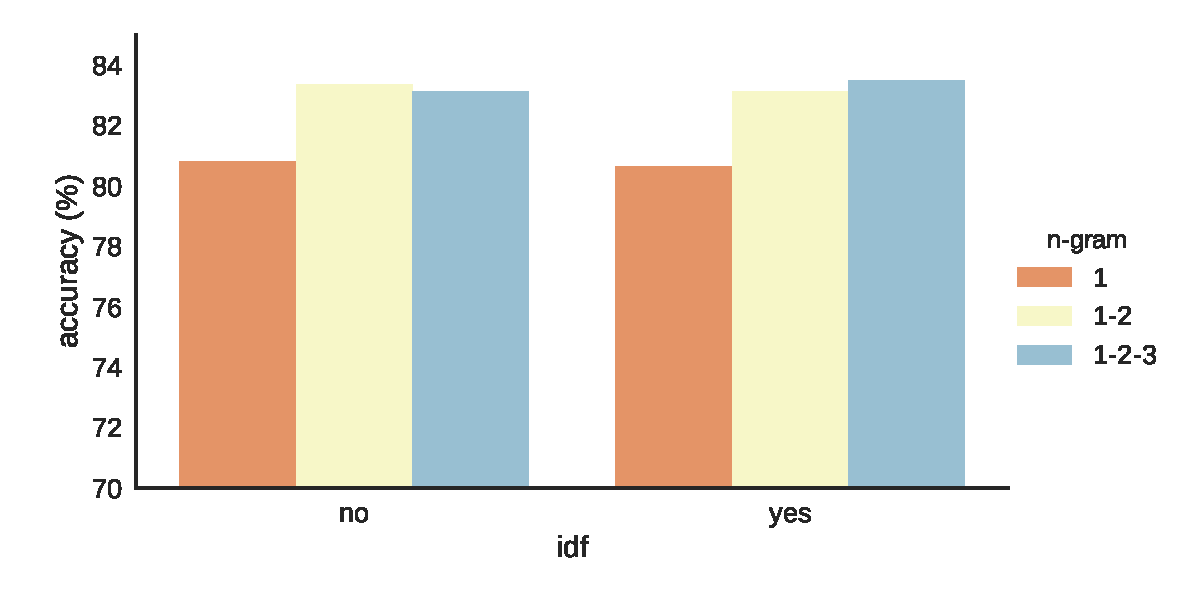
\includegraphics[width=\linewidth]{imag/idf.pdf}
    \caption{Accuracies of logistic regression using bags of words as input.}
    \label{fig:my_label}
\end{figure}
%\begin{table}
%\begin{center}
%\begin{tabular}{|c|c|c|c|}
%\hline
%Model & k-grams & $idf$ & accuracy \\
%\hline
%Logistic regression & 1 & No & 80.80\% \\
%\hline
%Logistic regression & 1, 2 & No & 83.35\% \\
%\hline
%Logistic regression & 1, 2, 3 & No & 83.12\% \\
%\hline
%Logistic regression & 1 & Yes & 80.63\% \\
%\hline
%Logistic regression & 1, 2 & Yes & 83.14\% \\
%\hline
%Logistic regression & 1, 2, 3 & Yes & 83.49\% \\
%\hline
%\end{tabular}
%\label{accuracies_bow}
%\caption{Accuracies of different models using bags of words as input.}
%\end{center}
%\end{table}

We can remark that considering orders in the tokens improves the accuracy by almost 3\%.

Finally, we can see two main directions in which we can try to improve. The first one is the representation of words. As our representation is sparse and very high dimensional, we do not take advantage that some words can be semantically near. Embeddings that we are going to use in the next section tackle this issue. The second direction is the sequential aspect of text. Considering, the order of words seems very important. We inject some order using k-grams but due to combinatorial explosion, we can not take many of them. To address this problem, we will use convolutional neural networks.


\subsection{Deep representations}
\section{Convolutional networks and embeddings}

\subsection{Tweet representation}

Thanks to the preprocessing, we have clean tweets that have a far smaller vocabulary than the initial tweets. One of the main constraint to use neural networks for classification is to have a fixed input size. Thanks to the keras library we can easily build these sequences. We set the limit to 35 words as after the preprocessing, the majority of the tweets are under this limit. We do not want to set it to the maximum length of any tweet because it would lead to too many tweets with much zero padding resulting in very low performance.

Then we inspired ourselves of GloVe and Word2Vec and began all our models with an embedding layer which will learn a vector representation of our words.

Our baseline was done without any initialization.

Then we initialized it with the GloVe trained on 2 billions of tweets from Stanford, but let the possibility to this layer to train, because thanks to it we would get both a general information about the meaning of this particular word, and a specialization on our dataset. It is also necessary as some of our words were not found in the pretrained GloVe model.

\subsection{Models}

Convolutional neural networks are very popular to deal with natural language. It makes sense because group of words have usually more impact than words, and the position in the tweet of those group of words do not often matter.
As in the lecture and the whole literature on the Internet, we add a max pooling layer (subsampling) right after a convolution layer.

It is also interesting to stack those convolutional layers as group of words can also have interactions and a meaning.

We end our networks by a fully connected layer and a final layer with a single neuron performing the classification, that is to say returning a value between 0 and 1 which can also be interpreted as a confidence, even if we have a sigmoid the last layer.

As we are performing a binary classification, we set the loss function to binary crossentropy. We also use the Adam optimizer, described as very efficient for binary classification.

For the training, we observed than epochs after the $2^{nd}$ do not add much value to our accuracy.

\subsection{Results}

All different combination of layers led us to accuracies between 85\% and 86\%.

\section{Other Stuff}
\begin{figure}[h]
    \centering
    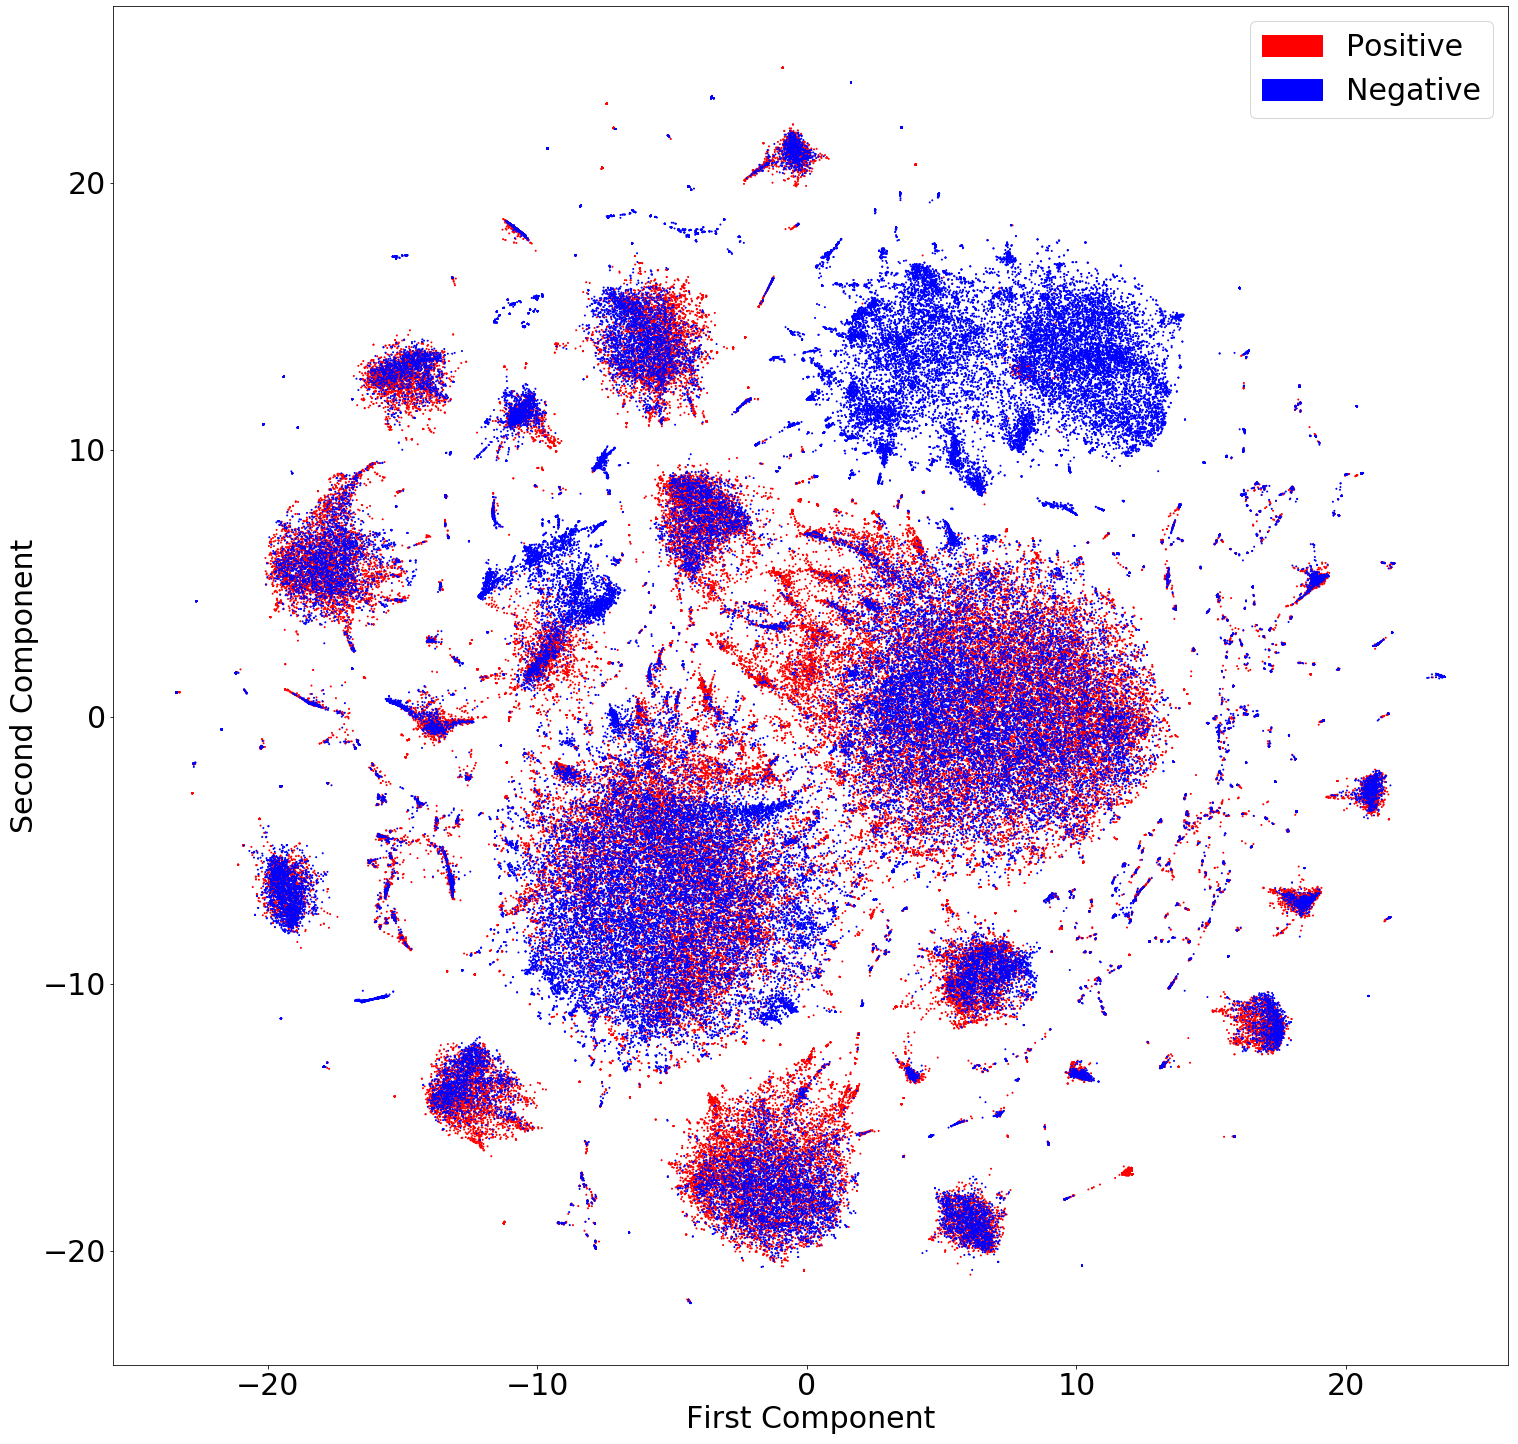
\includegraphics[width=\linewidth]{imag/tweets_tsne.png}
    \caption{TSNE visualization of embedded tweets by polarity}
    \label{fig:my_label}
\end{figure}

\subsection{Aggregation of several models}

As many of our models had reasonably high but different results, we thought than an average or a vote between different would perform best than every single model. Instead of a simple average, we chose to implement a classifier, which takes as features the outputs of all our different models. We tried several approaches for this purpose : 
\begin{table}[h]
\begin{center}
\begin{tabular}{|c|c|c|c|}
\hline
Model & accuracy \\
\hline
Random Forests & 81.60\% \\
\hline
AdaBoostClassifier & 86.280\% \\
\hline
Logistic regression & 86.540\% \\
\hline

\end{tabular}
\label{classifier}
\caption{Accuracies of final classifiers to aggregate our best models.}
\end{center}
\end{table}


\section{Conclusion}

\end{document}